\chapter{Spin Analysis}
\label{chap:spin}
\chapterquote{In a spin, loving the spin I'm in.}{Louis Prima, 1910--1978}

The Landau-Yang theorem forbids the direct decay of a spin-1 particle into a pair of photons~\cite{Landau1948,Yang1950}. 
Consequently the spin analysis compares the expectation of the spin-0 SM Higgs, \zerop, and the spin-2 \emph{graviton-like} 
model with minimal couplings, \twomp,~\cite{Gao2010}. The \twomp graviton resonance is produced in one of two ways, gluon-fusion ($gg$) 
or quark-antiquark annihilation (\qqbar). This chapter presents hypothesis tests between the \zerop and the \twomp varying the the amount of 
\twomp production from \qqbar. For the \zerop SM 
resonance all production modes have been considered; \ggH, \VBF, \WH, \ZH, \ttH. 

As the \twomp is just one of many spin-2 models it is desirable to make the analysis as model independent as possible. As a means of 
discriminating the two hypotheses we use the scattering angle in the Collins-Sopper frame, \costhetastar ~\cite{CollinsSoper1977}, which is defined as the angle, in the diphoton rest frame, between the collinear diphotons 
and the line which bisects one incoming beam with the negative of the other beam, 
\begin{equation}
  \cos(\theta^{\ast}_{\mbox{\tiny{CS}}}) = 2\times\frac{E_{2}p_{z1}-E_{1}p_{z2}}{m_{\gamma\gamma}\sqrt{m^{2}_{\gamma\gamma}+p^{2}_{T\gamma\gamma}}},
\end{equation}
where $E_{1}$ and $E_{2}$ are the energies of the leading and trailing photon, $p_{z1}$ and $p_{z2}$ are the $z$-component momenta 
of the leading and trailing photon and $m_{\gamma\gamma}$ and $p_{T\gamma\gamma}$ are the invariant mass and transerve momenta of the diphoton system.

In its rest frame the photons from the decay of a spin-0 boson are isotropic. Hence prior to acceptance cuts, the distribution of \costhetastar 
under the \zerop hypothesis is uniformly flat. In general this is not the case for spin-2 decays. 

In order to reduce any model dependence in the analysis the cut based photon selection, described in Sec.~\ref{sec:cic}, is used to pick events. The \MVA methods used for event selection in the nominal analysis use specific \SM \MC training samples and most importantly one of the training variables used, namely $\cos(\phi_{1}-\phi_{2})$, is highly correlated to the angular variable, \costhetastar, which can be used to distinguish spin hypotheses. Furthermore, given the unusual production modes of a spin-2 boson, no exclusive tagging is used in the spin analysis. The impact of using jet variables was studied but it was found that the sensitivty for distinguishing spin hypotheses was improved by a neglible amount.

Two statistical tests are carried out in the spin analysis:

\begin{enumerate}
  \item The signal strength, $\mu$, is extracted differentially in bins of \abscostheta. This is a relatively model independent test and in principal allows any spin model to be compared to the data.
  \item The statistical separation between different spin hypotheses is calculated using a test statistic similar to the one described in Sec.~\ref{sec:stats} and the $CL_{s}$ exclusion method is used to quantify the separation power. This is a highly model dependent test but allows for the exclusion of specific spin models.
\end{enumerate}

\section{Event categorisation}
\label{sec:spin_cats}

%Preceding the cut based selection mentioned in section \ref{sec:photonID} and described in Ref.~\cite{HIG-13-001}, photons
%are preselected requiring, $p_{T}/m_{\gamma\gamma}>1/3$ ($p_{T}/m_{\gamma\gamma}>1/4$) for the leading (subleading) photon and
%$|\eta_{\mbox{\tiny{cluster}}}|<2.5$ for all photons, where $p_{T}$ is the transverse momentum of a photon, $m_{\gamma\gamma}$ is the diphoton invariant mass and $|\eta_{\mbox{\tiny{cluster}}}|$ is the pseudorapidity of the photon supercluster. In addition photons are rejected whose supercluster lies within the barrel-endcap transition region, $1.4442<|\eta_{\mbox{\tiny{cluster}}}|<1.566$.
The effect of the photon selection cuts on the distributions of 
\abscostheta is illustrated in Fig.~\ref{fig:acc_cuts}. Before any acceptance cuts, Fig.~\ref{fig:acc_cuts} (left), the \abscostheta
distribution of the \zerop processes is flat. This is not the case for the \twomp processes (gluon-fusion and quark-antiquark annihilation). After the selection cuts are applied these distributions are considerably distorted, Fig.~\ref{fig:acc_cuts} (right). As a Higgs produced from vector-boson-fusion, which is $\sim$8\% of the total (compared to $\sim$88\% from gluon fusion),  is typically produced at higher transverse momentum there is some additional contribution of \zerop signal at high values of \abscostheta compared to the \twomp production modes after the selection cuts.

\begin{figure}
	\begin{center}
	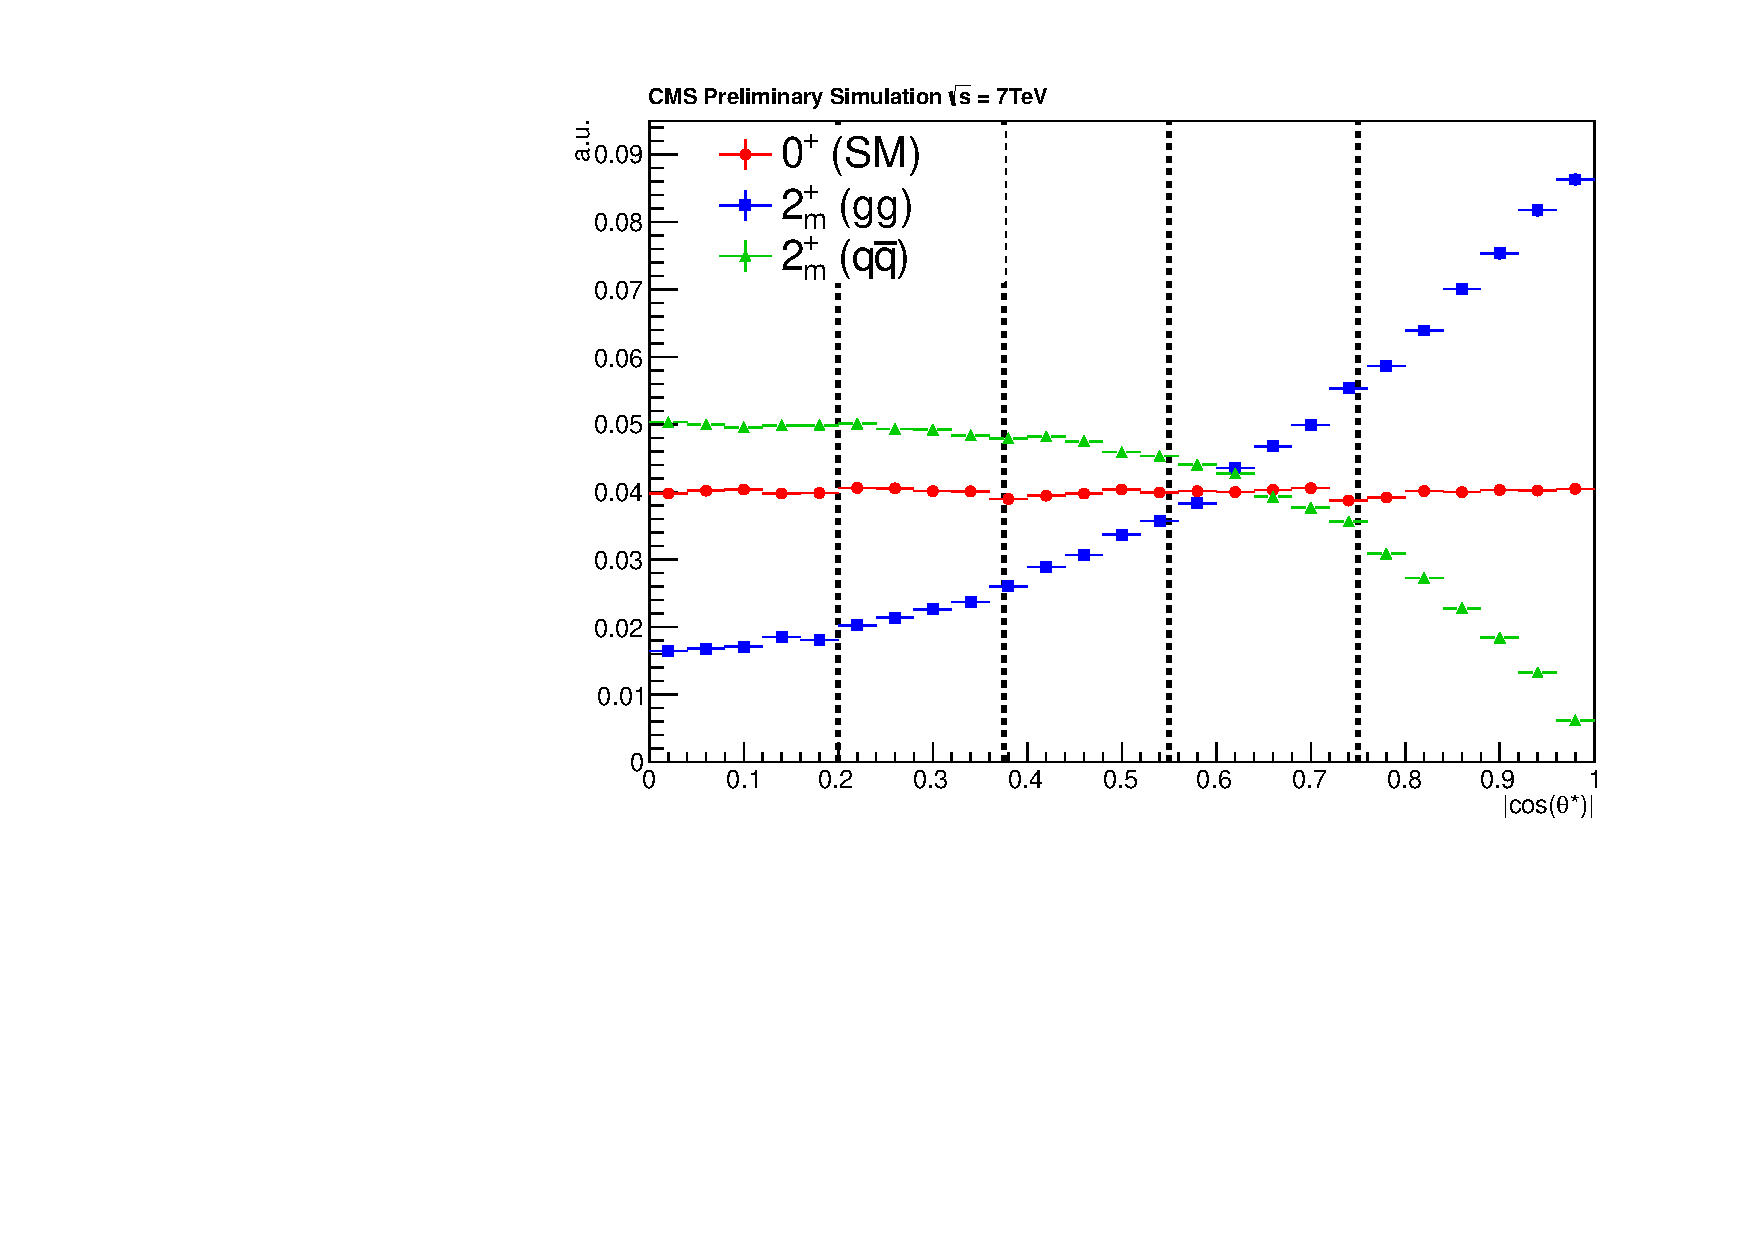
\includegraphics[width=0.49\linewidth]{spin/plots/before_7TeV.pdf}
	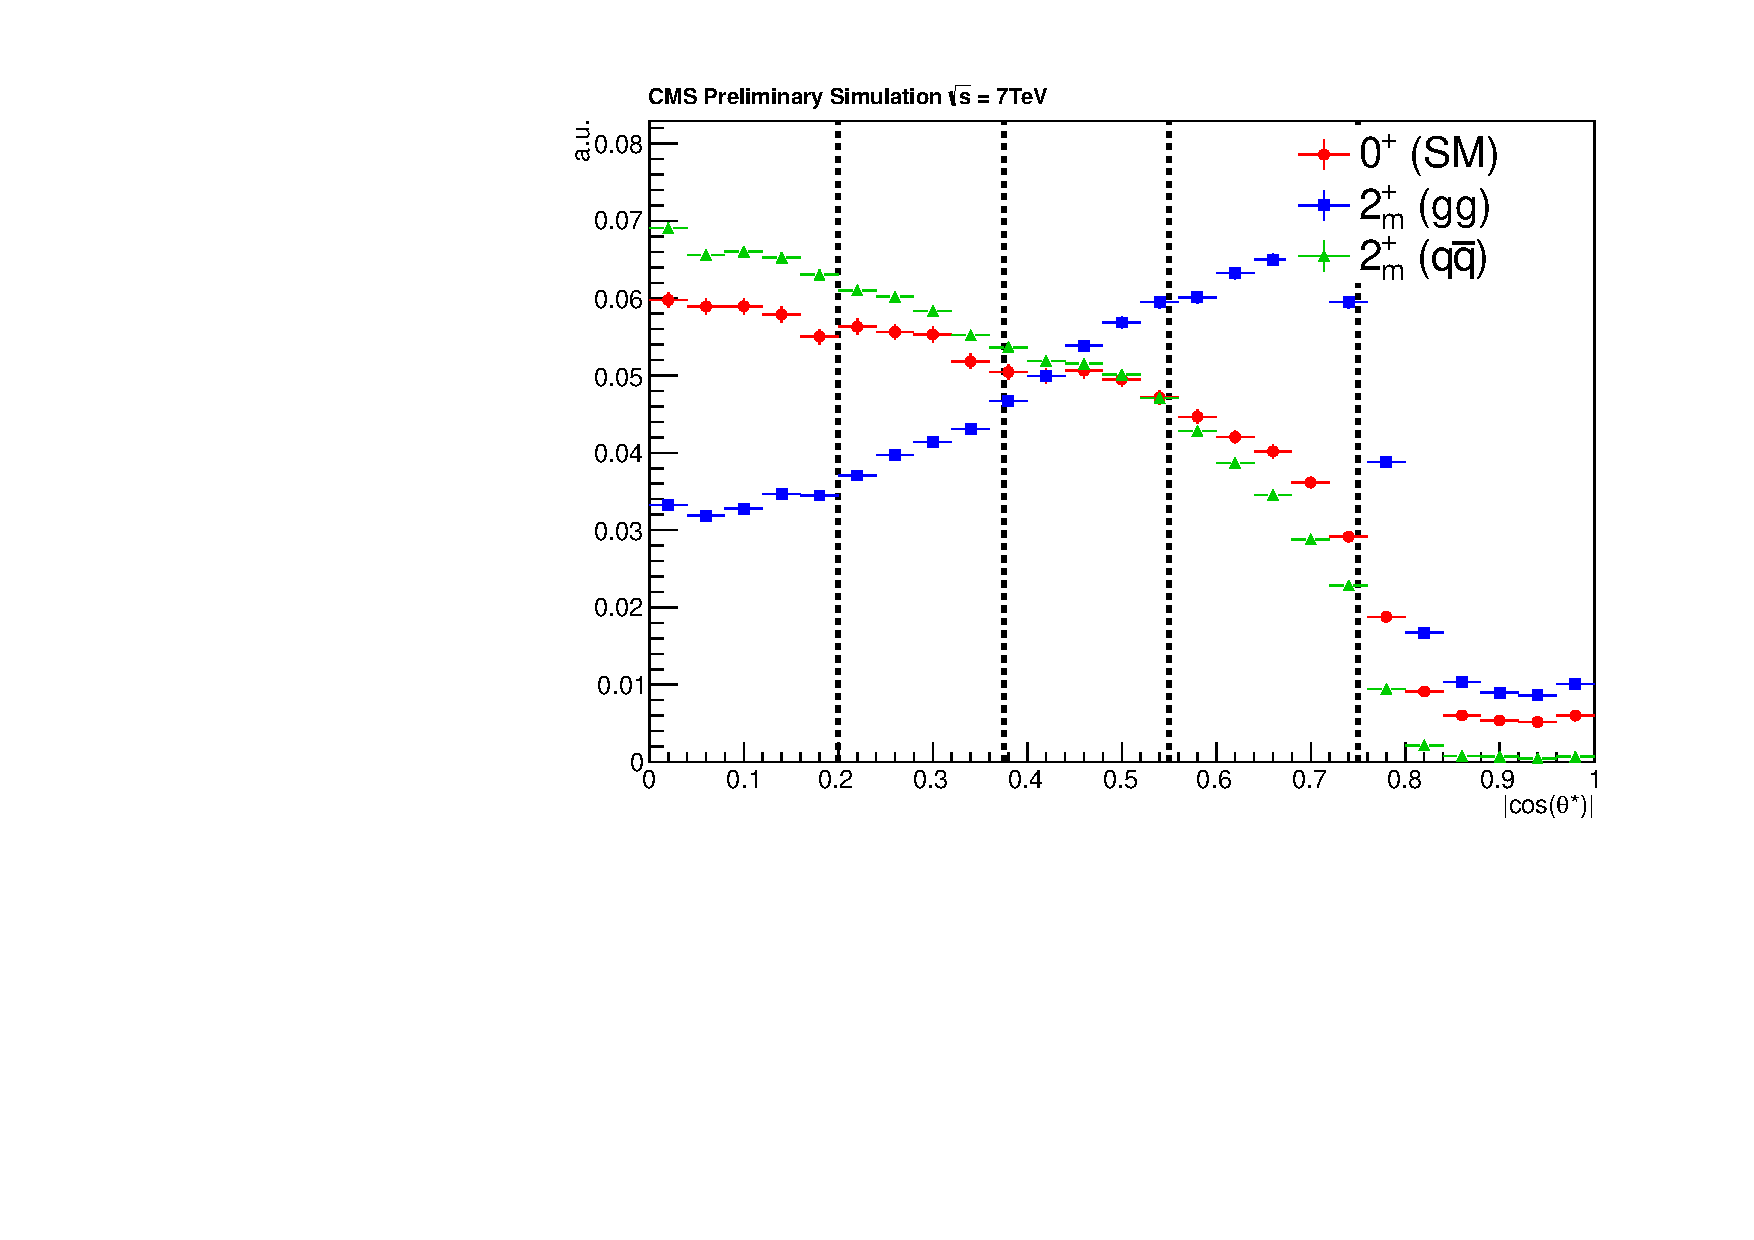
\includegraphics[width=0.49\linewidth]{spin/plots/after_7TeV.pdf} \\
	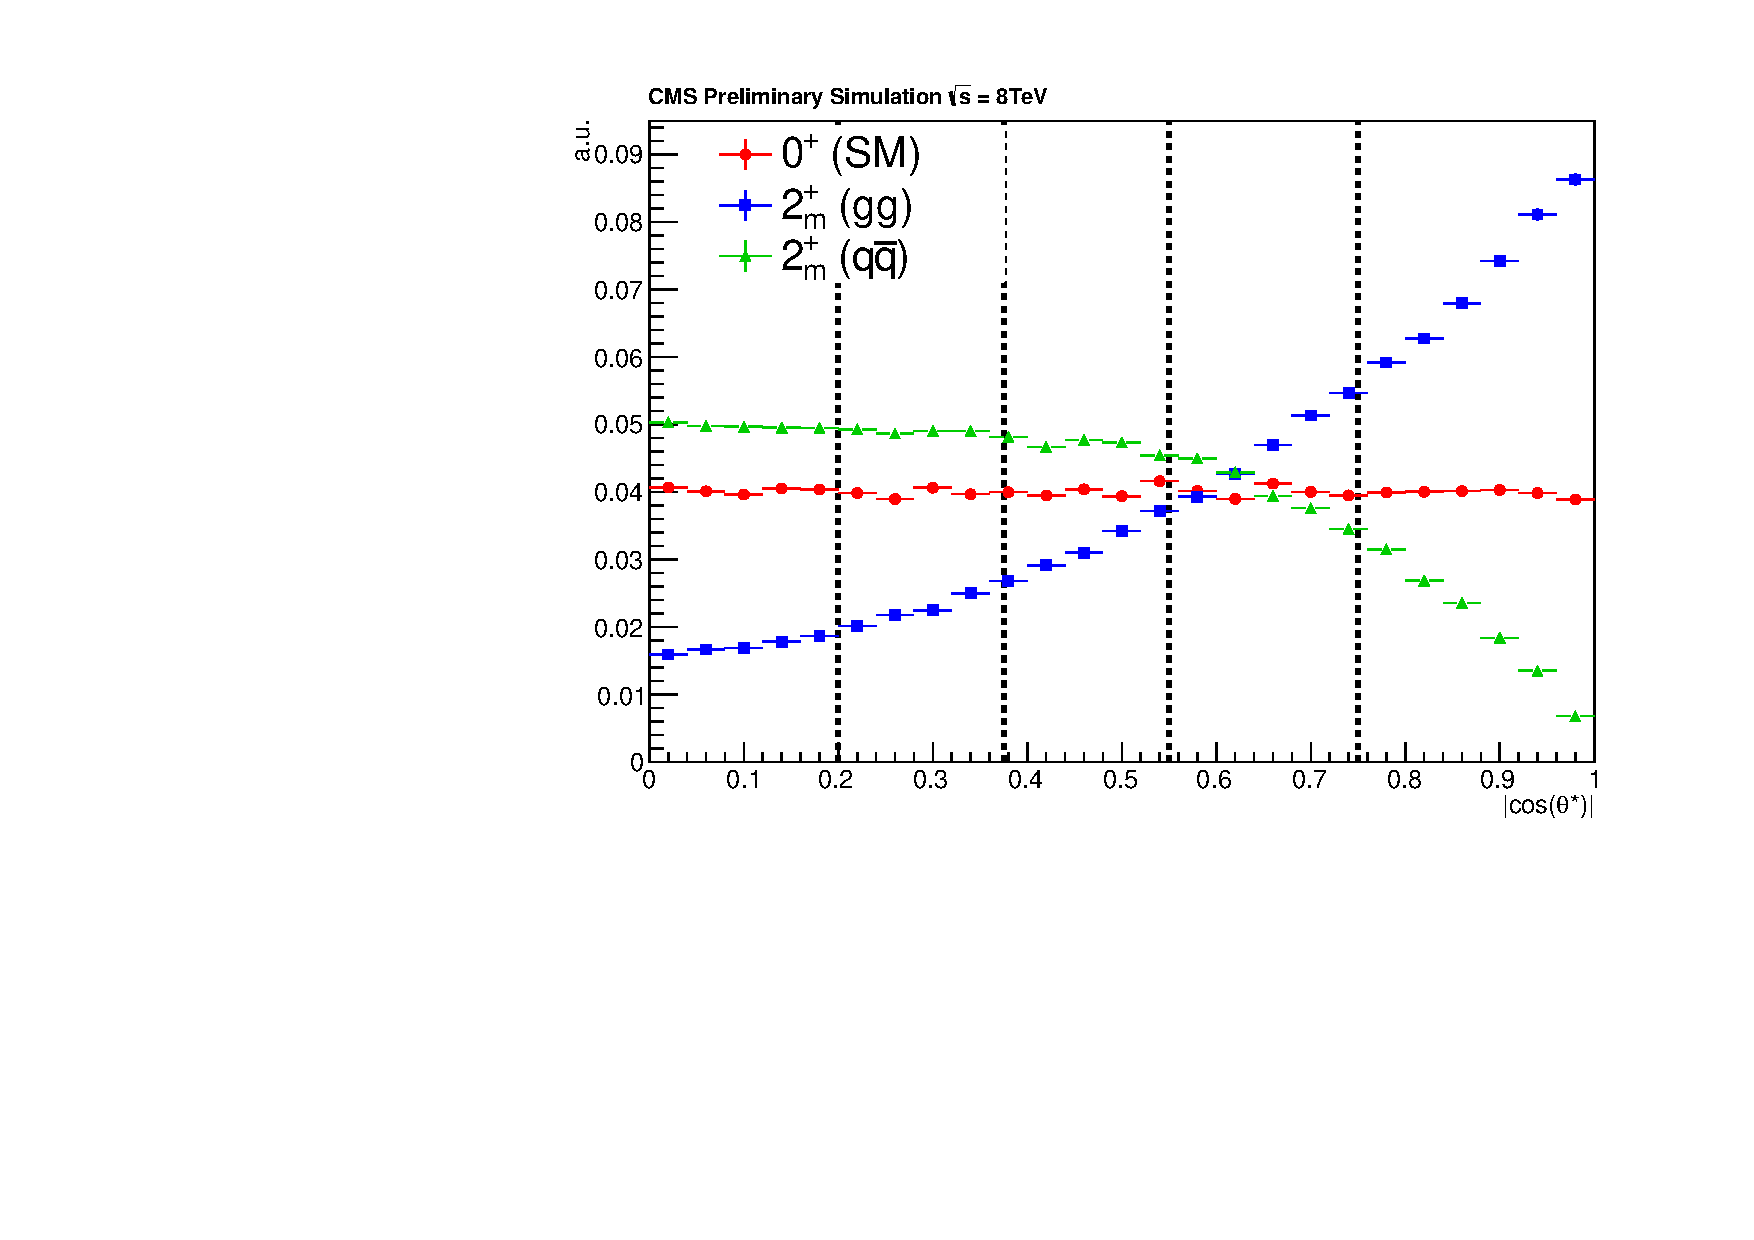
\includegraphics[width=0.49\linewidth]{spin/plots/before_8TeV.pdf}
	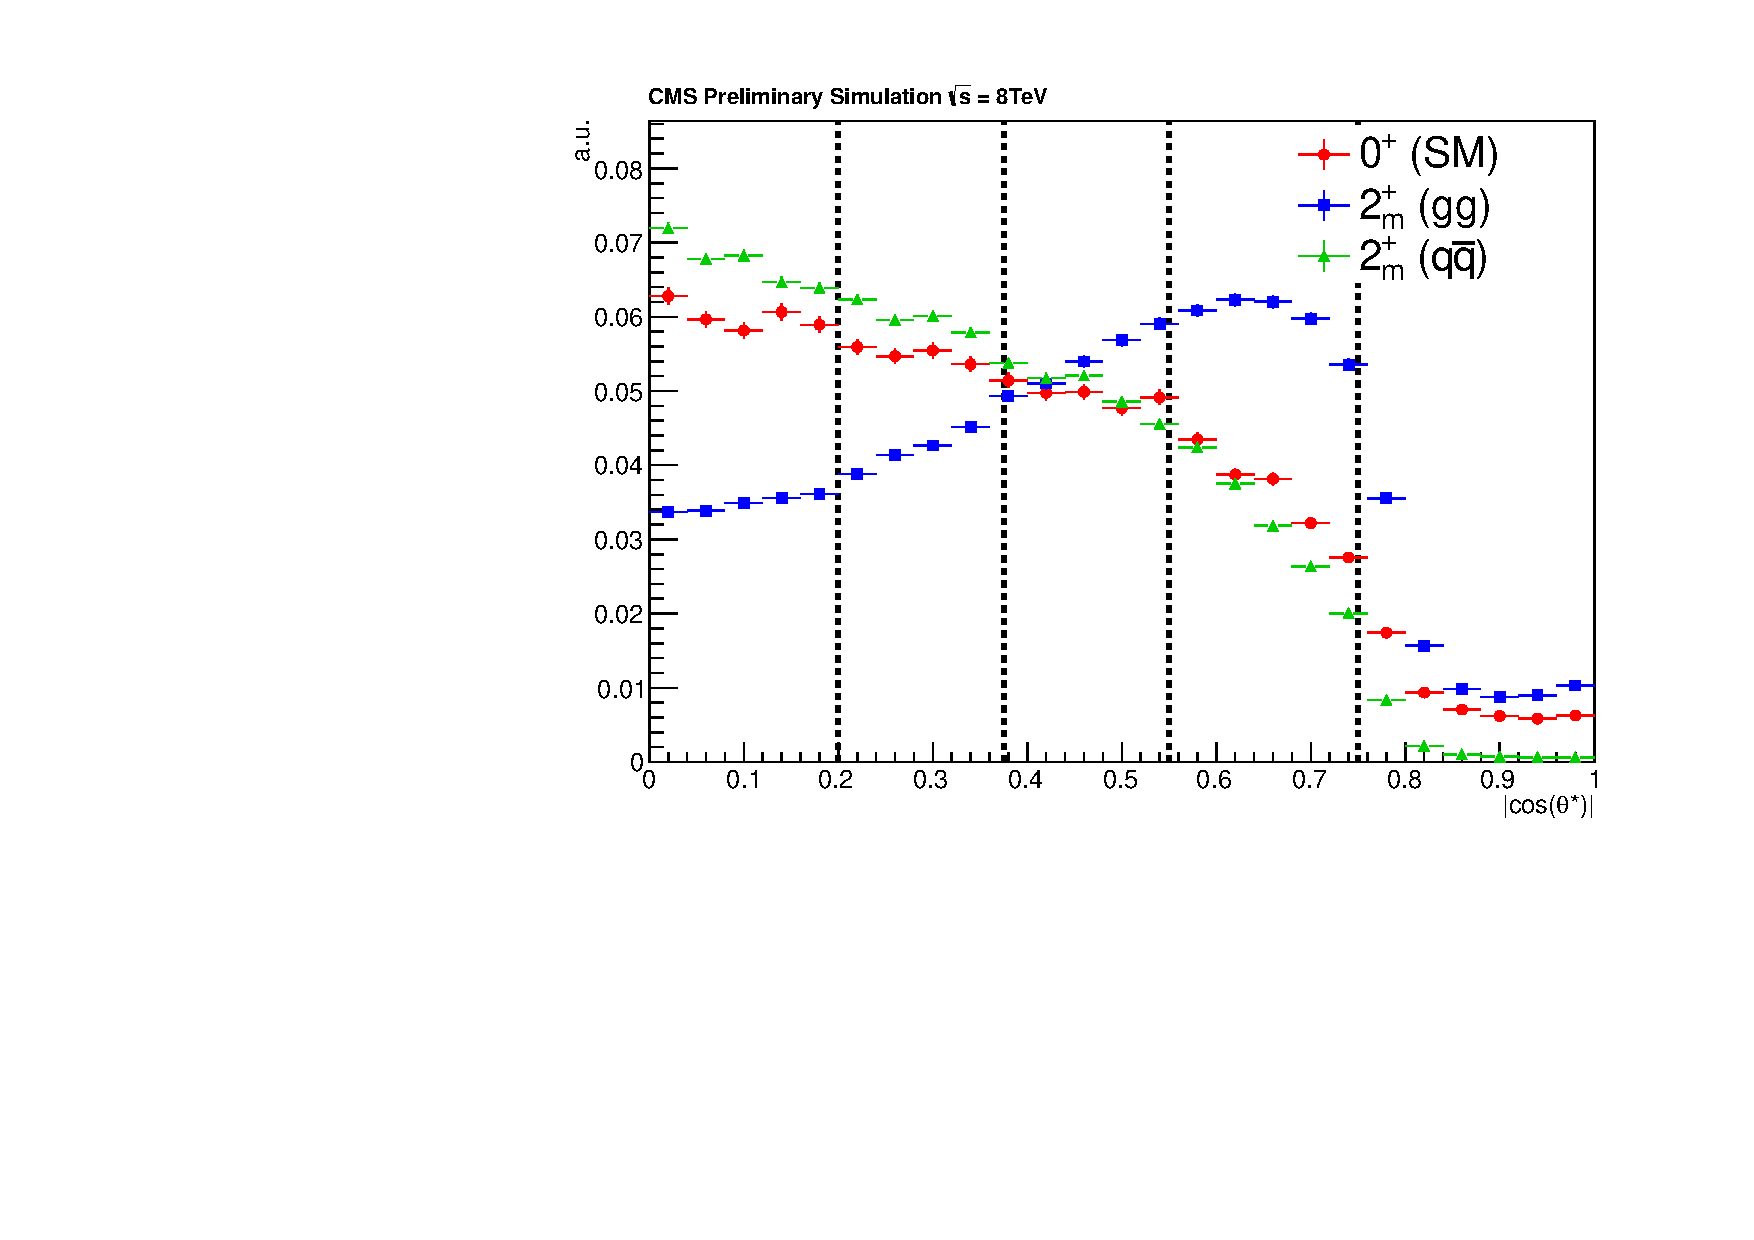
\includegraphics[width=0.49\linewidth]{spin/plots/after_8TeV.pdf} \\
	\caption{The distribution of \abscostheta before any selection cuts (left) and after the selection cuts (right) for the 7~\TeV dataset top row and the 8~\TeV dataset bottom row. The three histograms represent the spin $0^+$ distribution with all SM production modes (red circular points), the spin $2^+_m$ distribution with the gluon-fusion production mode (blue square points) and the spin $2^+_m$ distribution with the quark-antiquark annihilation production mode (green triangular points). The \abscostheta category boundaries are shown as the black dashed lines.}
	\label{fig:acc_cuts}
	\end{center}
\end{figure}	

A robust analysis is possible because although the acceptance $\times$ efficiency varies considerably as a function of \abscostheta, the shape of this variation is largely independent of the spin-parity model. This is also true in restricted ranges of $\eta$ and $R_{9}$ which allows us to extract the signal yield in bins of \abscostheta in a comparatively model independent way. 
Figure~\ref{fig:eff_acc} shows the efficiency $\times$ acceptance ratio between the \twomp (with gluon-fusion production only) and \zerop (all SM production modes) as a function of \abscostheta in the $|\eta|$ and $R_{9}$ categories defined in Table~\ref{table:cats1}. It is clear that the acceptance $\times$ efficiency between the spin-0 and spin-2 models is independent of \abscostheta apart from at high values of \abscostheta where the vector-boson-fusion production in the SM plays a role. This motivates the choice of \abscostheta category boundaries described below where all the categories have similar efficiency $\times$ acceptance apart from the bin highest in \abscostheta.

\begin{figure}
	\begin{center}
	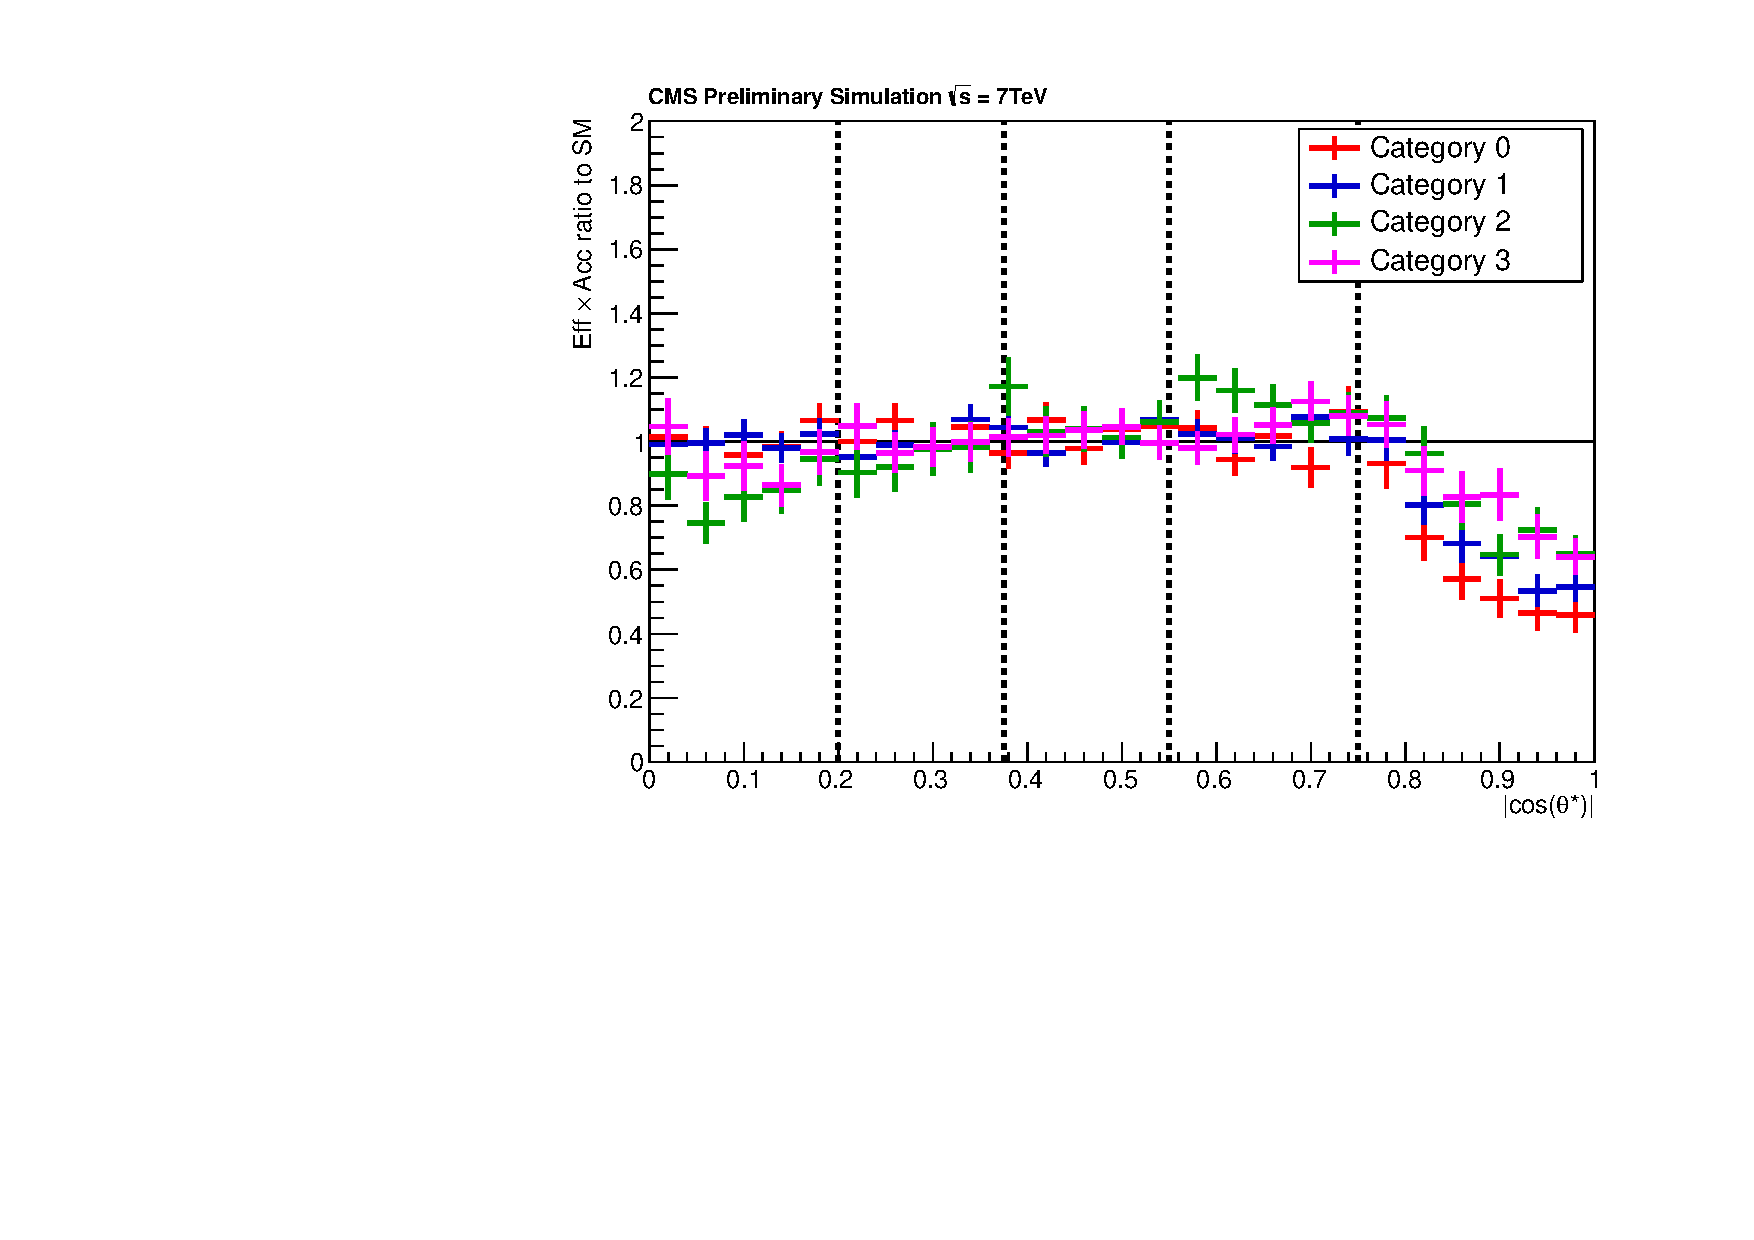
\includegraphics[width=0.49\linewidth]{spin/plots/effacccats_7TeV.pdf}
	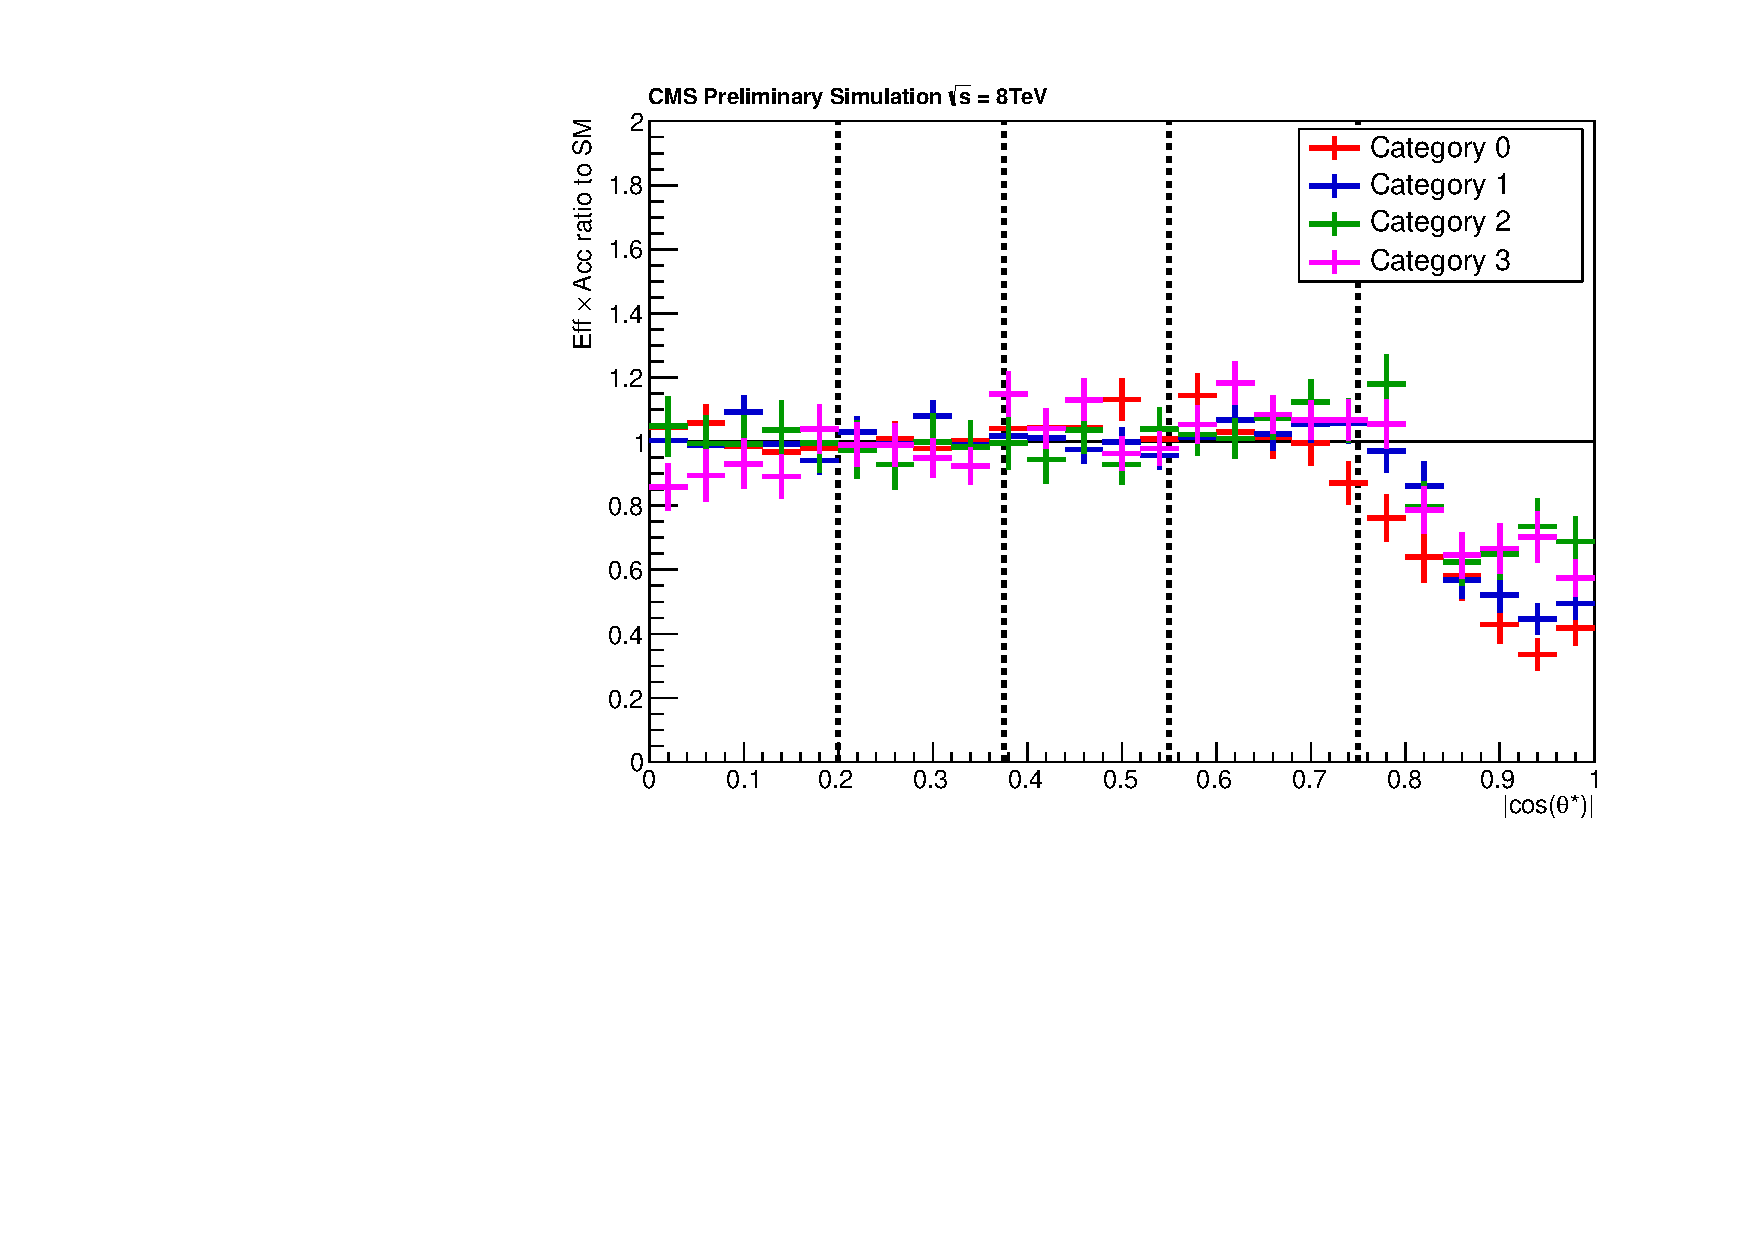
\includegraphics[width=0.49\linewidth]{spin/plots/effacccats_8TeV.pdf}
  \caption{Acceptance $\times$ efficiency ratio between the \twomp (gluon-fusion production) and \zerop (all SM production modes) of the event selection as a function of \abscostheta split into the $|\eta|$ and $R_{9}$ categories defined in Table.~\ref{table:cats1}. The \abscostheta category boundaries are shown as the black dashed lines. The left hand plot is for the 7~\TeV \MC and the right hand plot for the 8~\TeV.}
	\label{fig:eff_acc}
	\end{center}
\end{figure}	


To benefit from the improved energy resolution of non-showering photons in 
the barrel, each event is categorised in $\eta$ and $R_{9}$ according to Table~\ref{table:cats1}.

\begin{table}
  \begin{center}
    \begin{tabular}{| l | l l l |}
      \hline
      Category 0 & $|\eta|_{\mbox{\tiny{max}}}<1.5$ & and & $R_{9\mbox{\tiny{min}}}>0.94$ \tabularnewline 
      Category 1 & $|\eta|_{\mbox{\tiny{max}}}<1.5$ & and & $R_{9\mbox{\tiny{min}}}\leq0.94$ \tabularnewline 
      Category 2 & $|\eta|_{\mbox{\tiny{max}}}>1.5$ & and & $R_{9\mbox{\tiny{min}}}>0.94$ \tabularnewline 
      Category 3 & $|\eta|_{\mbox{\tiny{max}}}>1.5$ & and & $R_{9\mbox{\tiny{min}}}\leq0.94$ \tabularnewline
      \hline
    \end{tabular}
    \caption{Definition of photon resolution categories}
    \label{table:cats1}
  \end{center}
\end{table}

%\begin{tabular}{l l l l l}
%  \textbullet & Category 0: & $|\eta|_{\mbox{\tiny{max}}}<1.444$ & and & $R_{9\mbox{\tiny{min}}}>0.94$ \\ 
%  \textbullet & Category 1: & $|\eta|_{\mbox{\tiny{max}}}<1.444$ & and & $R_{9\mbox{\tiny{min}}}\leq0.94$ \\ 
%  \textbullet & Category 2: & $|\eta|_{\mbox{\tiny{max}}}>1.444$ & and & $R_{9\mbox{\tiny{min}}}>0.94$ \\ 
%  \textbullet & Category 3: & $|\eta|_{\mbox{\tiny{max}}}>1.444$ & and & $R_{9\mbox{\tiny{min}}}\leq0.94$ \\
%\end{tabular}

Within each category events are binned in \abscostheta, to discrimate between the different spin hypotheses, according to Table.~\ref{table:cats2}.

\begin{table}
  \begin{center}
    \begin{tabular}{| l | r l |}
      \hline
      Spin Category 0 &             & \abscostheta $<0.2$ \tabularnewline 
      Spin Category 1 & $0.2\leq$   & \abscostheta$<0.375$ \tabularnewline 
      Spin Category 2 & $0.375\leq$ & \abscostheta$<0.55$ \tabularnewline 
      Spin Category 3 & $0.55\leq$  & \abscostheta$<0.75$ \tabularnewline 
      Spin Category 4 & $0.75\leq$  & \abscostheta$<1.0$ \tabularnewline 
      \hline
    \end{tabular}
    \caption{Definition of photon \abscostheta categories}
    \label{table:cats2}
  \end{center}
\end{table}


The \abscostheta boundaries are optimised to make particular use of the most disciminating 
bin (high \abscostheta) and to maintain uniform acceptance $\times$ efficiency in the 
other bins. In total the analysis is split into 20 event classes (4 $\eta$/\rnine\xspace 
categories $\times$ 5 \abscostheta categories) in each year which gives a total of 40 event classes.

\section{Signal and Background modelling}

The signal models are obtained from \MC simulation as described in Sec.~\ref{sec:mc} for the spin-0 \SM processes and the spin-2 processes. A parametric model identical to the one built for the nominal analysis is constructed as per the method described in Sec.~\ref{sec:signal_mfm}. The signal model is then parametrised as before in terms of $\mu$, \mH and two additional parameters, $x$ and \fqqbar, which dictate the amount of signal from spin-2 and the amount of spin-2 from $q\bar{q}$ production. The signal model parametrisation can be written as,
\begin{equation}
  \textbf{S}(m_{H},fqq,x;\hat{\theta}) = (1-x)\cdot\boldsymbol{S_{SM}}(m_{H};\hat{\theta})  + x\cdot\Bigl[f_{q\bar{q}}\cdot \boldsymbol{S_{q\bar{q}}}(m_{H};\hat{\theta}) + (1-f_{q\bar{q}})\boldsymbol{S_{gg}}(m_{H};\hat{\theta})\Bigr],  
  \label{eq:spin_sig}
\end{equation}
where $x$ is the amount of signal originating from spin-2, \fqqbar is the amount of spin-2 signal originating from $q\bar{q}$ production, \mH is the signal position and $\theta$ are the nuisance parameters.

The background model for the spin analysis comes in two forms. For the differntial measurement of the signal strength in bins of \abscostheta the envelope background method is used as per the description in Sec.~\ref{sec:envelope}. However, when calculating the statistical separation between various spin hypotheses a single parametrisation of the background is used in each category, namely a polynomial in the Bernstein basis~\cite{bernsteins1,bernsteins2} as per the description in eq.~\ref{eq:bernsteins}. The reason for this is that there is no asymptotic approximation for the test statistic distribution when the null hypothesis is not embedded in the alternative hypothesis. Consequently, in order to obtain the test statistic distributions (like the ones shown in Fig.~\ref{fig:cls}) one has to generate lots of pseudo-data and then refit this data to obtain the likelihood ratio and hence test statistic value. Given the complexity of the spin signal model and the combinatorics involved when using the envelope method with 40 analysis categories this becomes CPU impractical. It has been trialled using the GRID computing network but was found to take the order of hundreds of CPU years.
Given this complication, and the fact that small losses in sensitivity to the background normalisation have a small impact on the spin hypothesis separation power, a single parametrisation in each category was chosen for ease and simplicity. The choice is to use 4th order Bernstein polynomials in all categories apart from the highest \abscostheta categories in which a 3rd order was chosen. The motivation behind this choice is that these order of polynomials show a similarly small level of bias as the envelope method when tested against ``truth" models for the spin categories analogous to the description in Sec.~\ref{sec:envelope}.

\section{Results}
\label{sec:spin_results}

The acceptance $\times$ efficiency of the two spin models in each category as well as the differential cross section as a function of \abscostheta, which depends only on the spin of the initial state, is obtained from the MC simulation. The only remaining assumption is on the total number of expected signal events for a given spin-parity state and production mode. This is well defined for the spin-0 SM case and is obtained from the $\sigma\times BR$ given by the LHC Higgs cross section working group in Ref.~\cite{LHCHiggsCrossSectionWorkingGroup3}. For the graviton-like \twomp this quantity is unknown. 
%Consequently, when generating pseduo-experiments for a particular model, the model is first fitted to the data to extract the relative shapes and normalisations of the signal and background. 
Consequently we scale the signal models for both spin hypotheses with a modifier, $\mu$, such that when $\mu=1$ and all \costhetastar information is ignored, the total number of expected signal events for the model in question is equivalent to the SM expectation. 
When generating pseduo-experiments for a particular model, the value of all the free parameters in the fit (including the signal nuisance parameters, the background shape parameters and the signal srength $\mu$) are set to their best fit values after fitting the model in question to the data.
In this way the expected separation is a fair representation of what we observe in data.

\subsection{SM compabibility check}
The signal yield, $\mu=\sigma/\sigma_{SM}$, is extracted independently in each of the \abscostheta bins, 
simultaneously fitting over the $\eta$ and \rnine bins such that the relative yields in each of the $\eta$ and \rnine 
bins is constrained to that predicted by the SM. The result is shown in Figure~\ref{fig:channelcomp} for the data (black points), the \zerop model expectation (red line), the \twomp model expectation using the $gg$ production mode only (blue line), the \twomp model expectation using the $q\bar{q}$ production mode only (green line) and the \twomp model expectation using a half-half mixture of $gg$ and $q\bar{q}$ production (magenta line), where for the expectations a single representative toy is used, obtained using asymptotic formulae from Ref.~\cite{asymptotic_form}, and the normalisation is extracted from a fit to data. The final point of the blue line can be understood
by referring back to Figure~\ref{fig:eff_acc}. The fact that the SM $ggH$ and $qqH$ production is of a similar strength at high values of \abscostheta causes the 
fitted strength (when fitting the \zerop model to the \twomp($gg$) expectation) to be smaller in the highest \abscostheta bin as compared to the second highest, contrary to what might be expected. 

\begin{figure}
  \begin{center}
    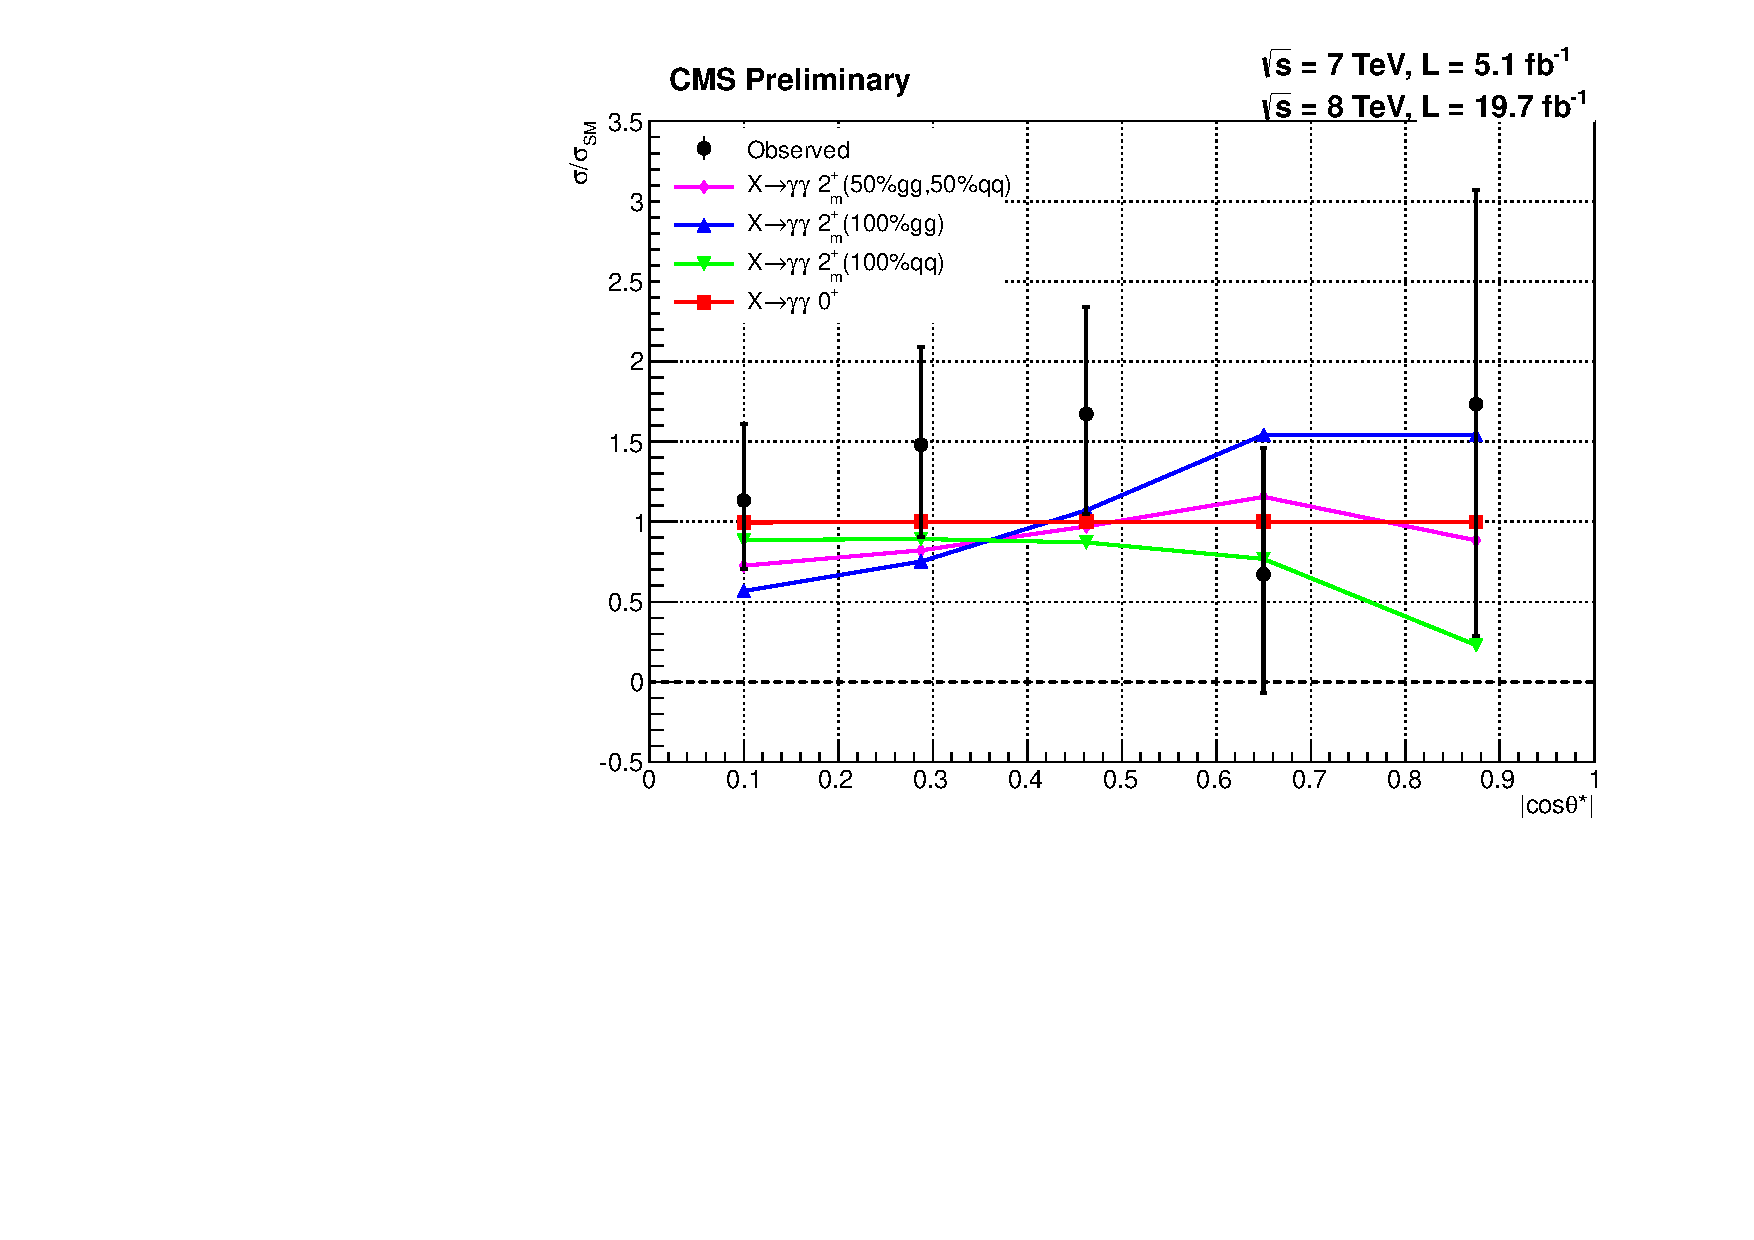
\includegraphics[width=0.8\linewidth]{spin/plots/ch_comp_multipdfcomb_unblind.pdf}
    \caption{The SM extracted signal yield as a function of \abscostheta for the \zerop expectation (red line), \twomp expectation with gluon-fusion production only (blue line), the \twomp expectation with quark-antiquark annihilation production only (green line), the \twomp expectation with half $gg$, half $q\bar{q}$ production (magenta line) and the observation (black points).}
    \label{fig:channelcomp}
  \end{center}
\end{figure}

\subsection{Hypothesis tests of the SM Higgs, \zerop, vs. graviton-like, \twomp}
\label{sec:spin_separation}

The separation between the two models and the data is extracted using the test statistic defined as twice the negative ratio 
of the likelihoods for the \zerop signal plus background hypothesis and the \twomp signal plus background hypothesis when 
performing a simultaneous fit of all twenty event classes together, $q=-2\,{\ln({\cal L}_{2^{+}_\mathrm{m} + \mathrm{bkg.}}/{\cal
L}_{0^+ + \mathrm{bkg.}})}$.

The distribution of this test statistic is shown in 
Fig.~\ref{fig:separation} for pseudoexperiments generated with an overall signal yield and signal position which is extracted from a fit to the data for
the \zerop hypothesis (orange) 
and the \twomp hypothesis (blue) for gluon-fusion production only (left) and quark-antiquark annihilation production only (right). The observed value is shown as the red arrow. The 1-$CL_{s}$ observed exclusion for a gluon-fusion only produced spin-2 boson is 93.7\% whilst for quark-antiquark produced boson is 85.0\%. 

\begin{figure}
  \begin{center}
    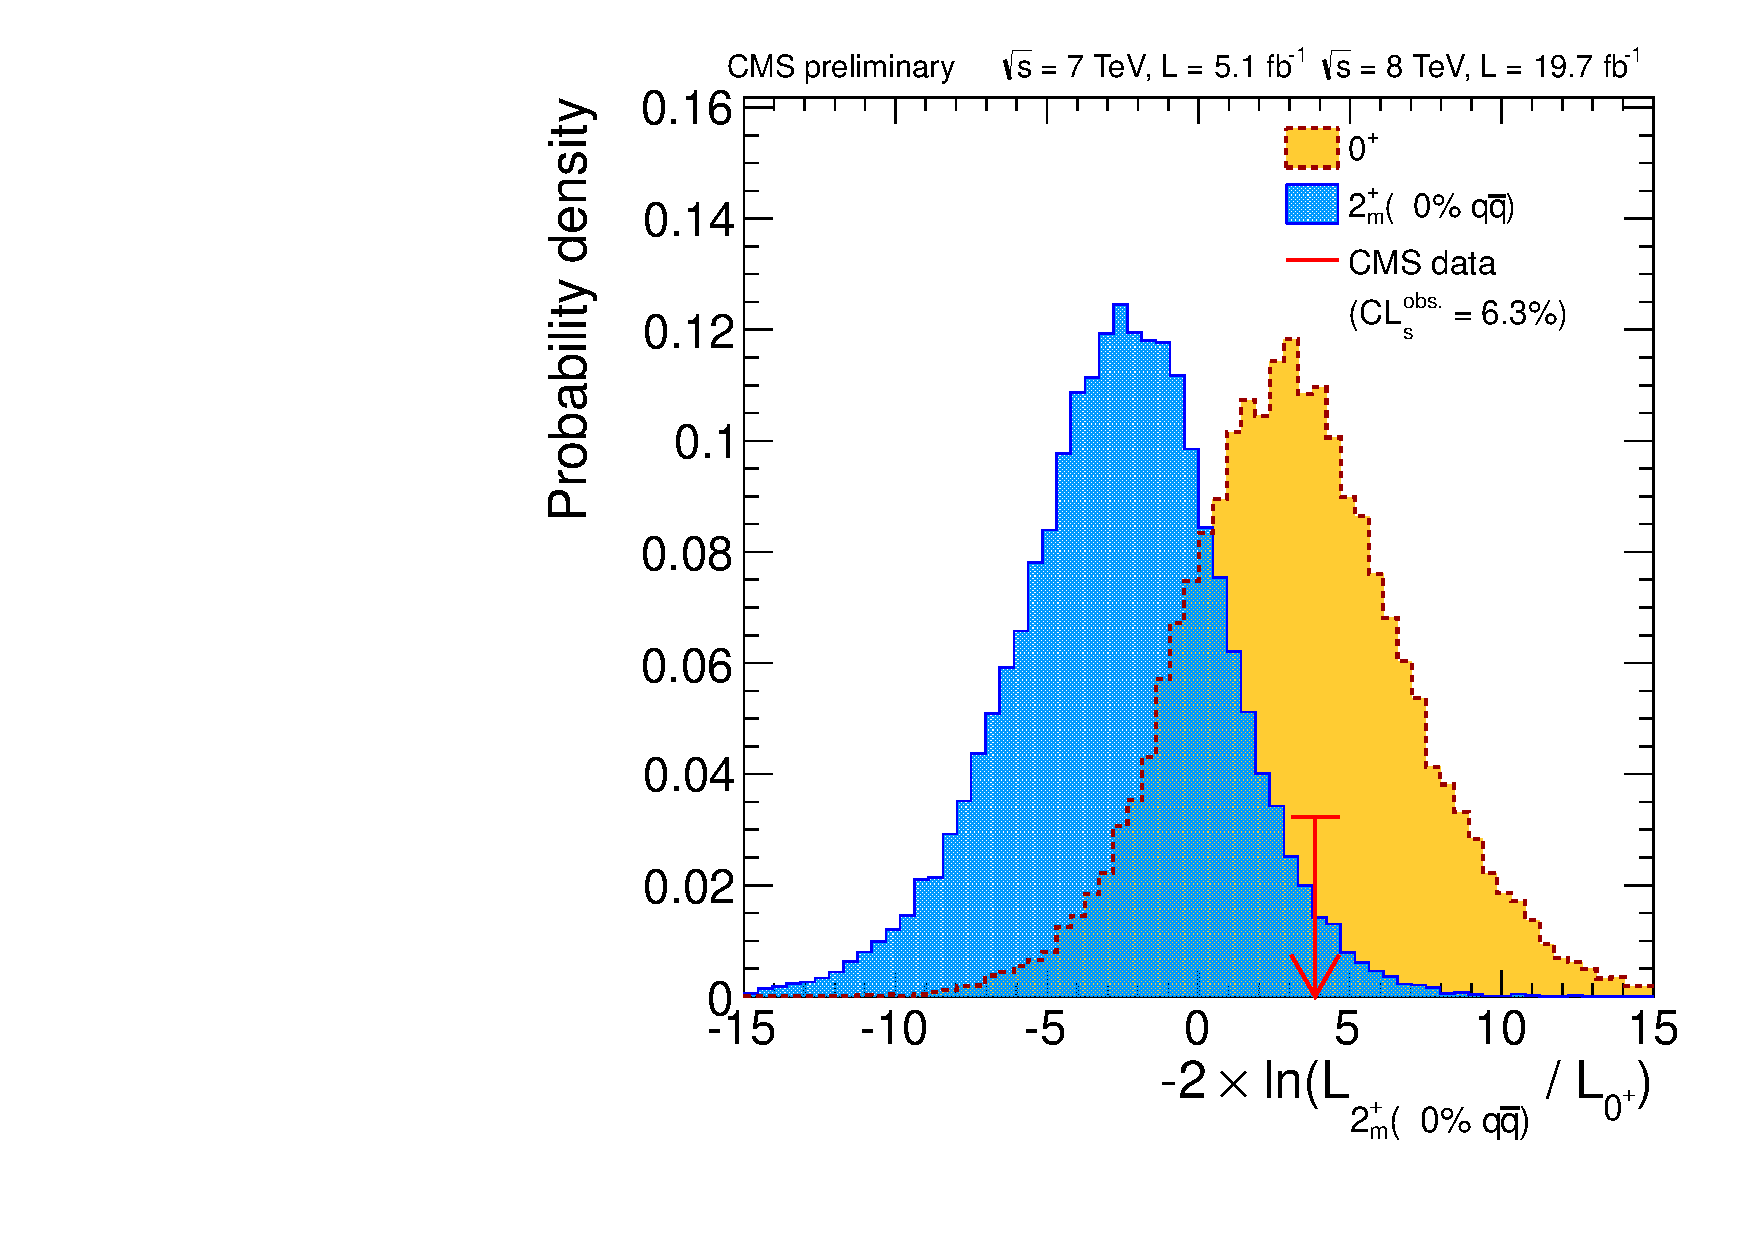
\includegraphics[width=0.49\linewidth]{{spin/plots/2pm0.00_unblind}.pdf}
    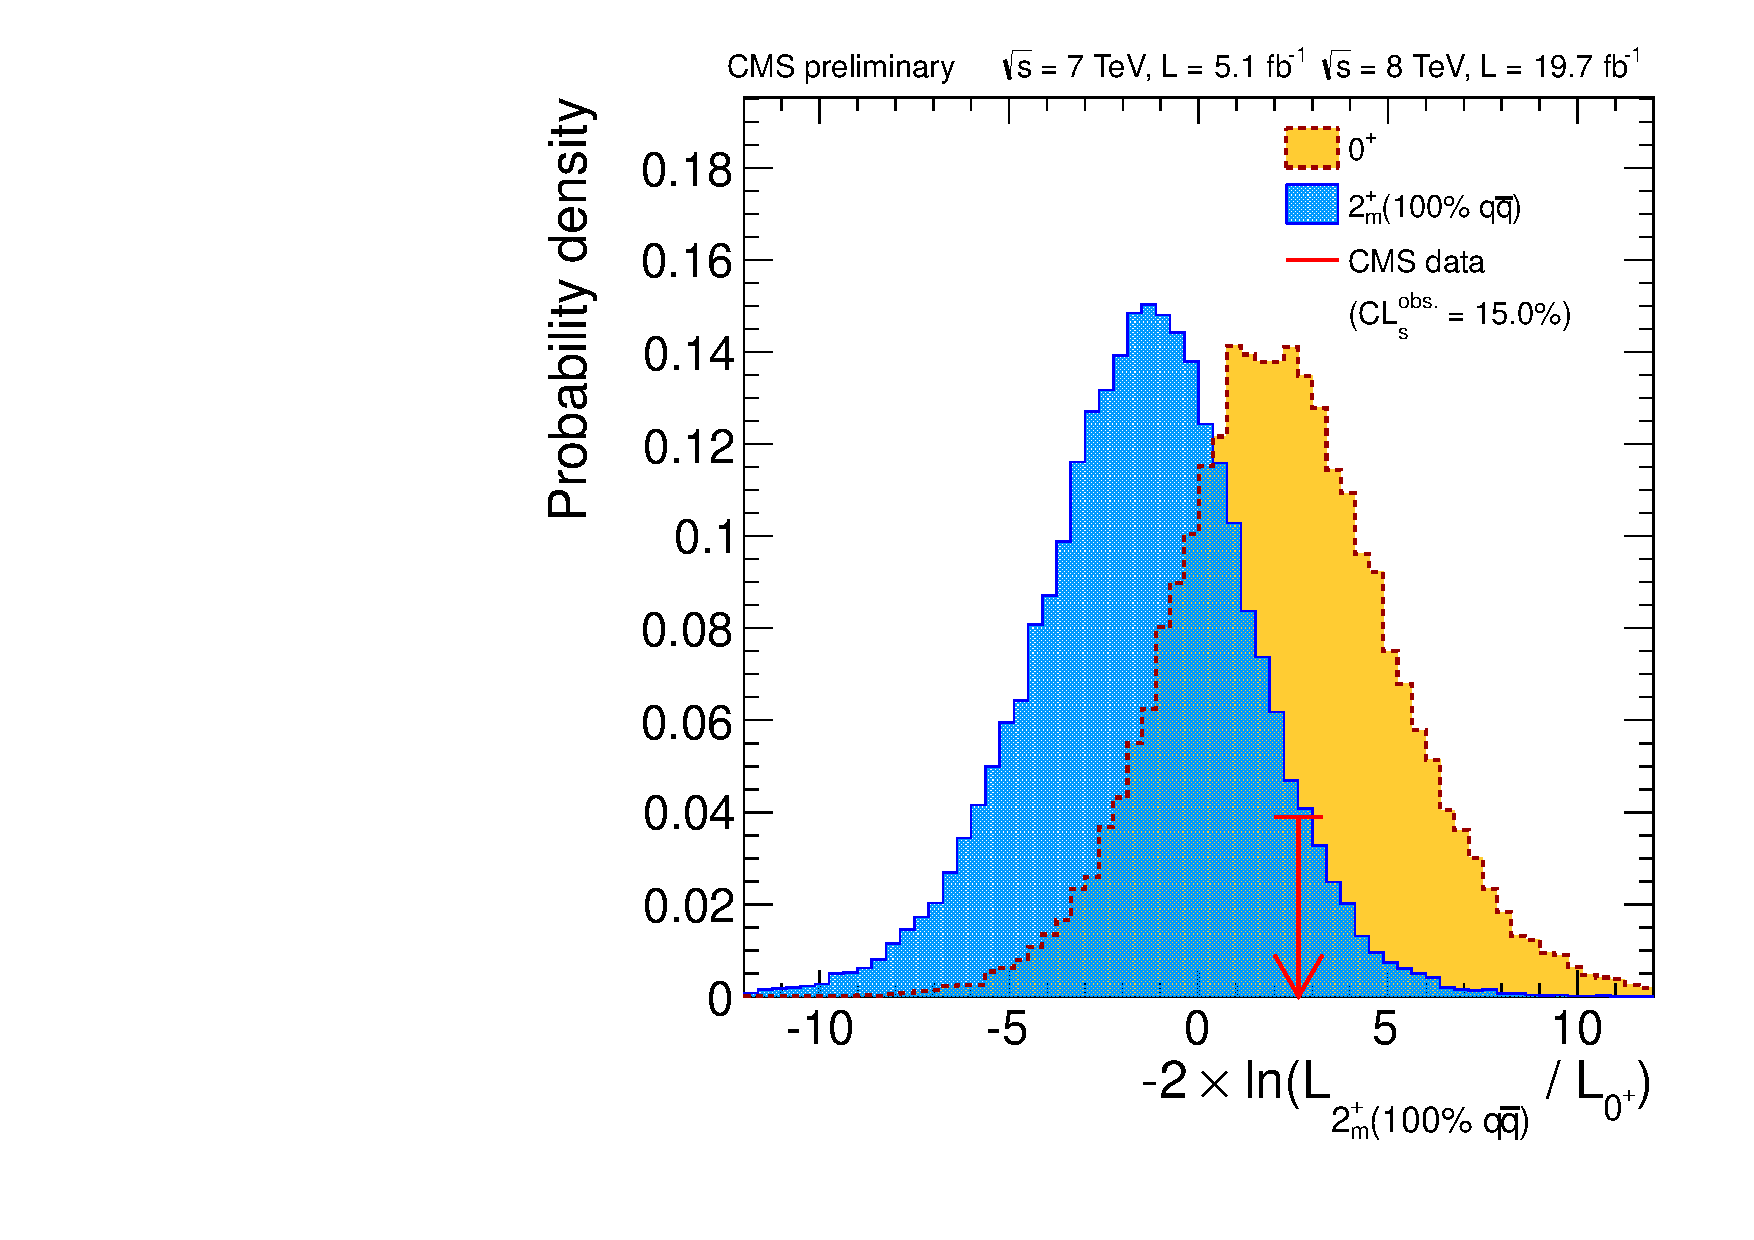
\includegraphics[width=0.49\linewidth]{{spin/plots/2pm1.00_unblind}.pdf}
    \caption{The distribution of the test statistic for pseudo experiments generated under the SM, \zerop, hypothesis (orange) and the \emph{graviton-like}, \twomp, hypothesis (blue) with gluon fusion produciton only (left) and quark-antiquark production only (right). The observed value in the data is shown as the red arrow.}
    \label{fig:separation}
  \end{center}
\end{figure}

The previous two tests are both performed assuming that the \twomp state is produced entirely by either gluon-fusion or quark-antiquark annihilation. A further three points, with mixtures of $gg$ and $q\bar{q}$ spin-2 production, have been tested such that the overall yield of the \twomp signal is fixed to the best fit value of the model in question to data and the fraction of \qqbar production is increased by a factor, \fqqbar. Figure~\ref{fig:qqbar} shows the distribution of the test statistic as a function of the fraction of \twomp production from $q\bar{q}$ annihilation. Figure~\ref{fig:separation} is, in effect, a projection of Fig.~\ref{fig:qqbar} at the points \fqqbar=0\% and \fqqbar=100\%. It can be seen that the data is very much in line with the \SM expectation. Whilst \textit{a prior} it may look as though the data points in Fig.~\ref{fig:qqbar} lie to close to the \SM mean (red line) all of these points are highly correlated. If the data look flat in \abscostheta then they will look flat for all values of \fqqbar. In this sense the green and yellow bands in Fig.~\ref{fig:qqbar} can be misleading.

\begin{figure}
  \begin{center}
    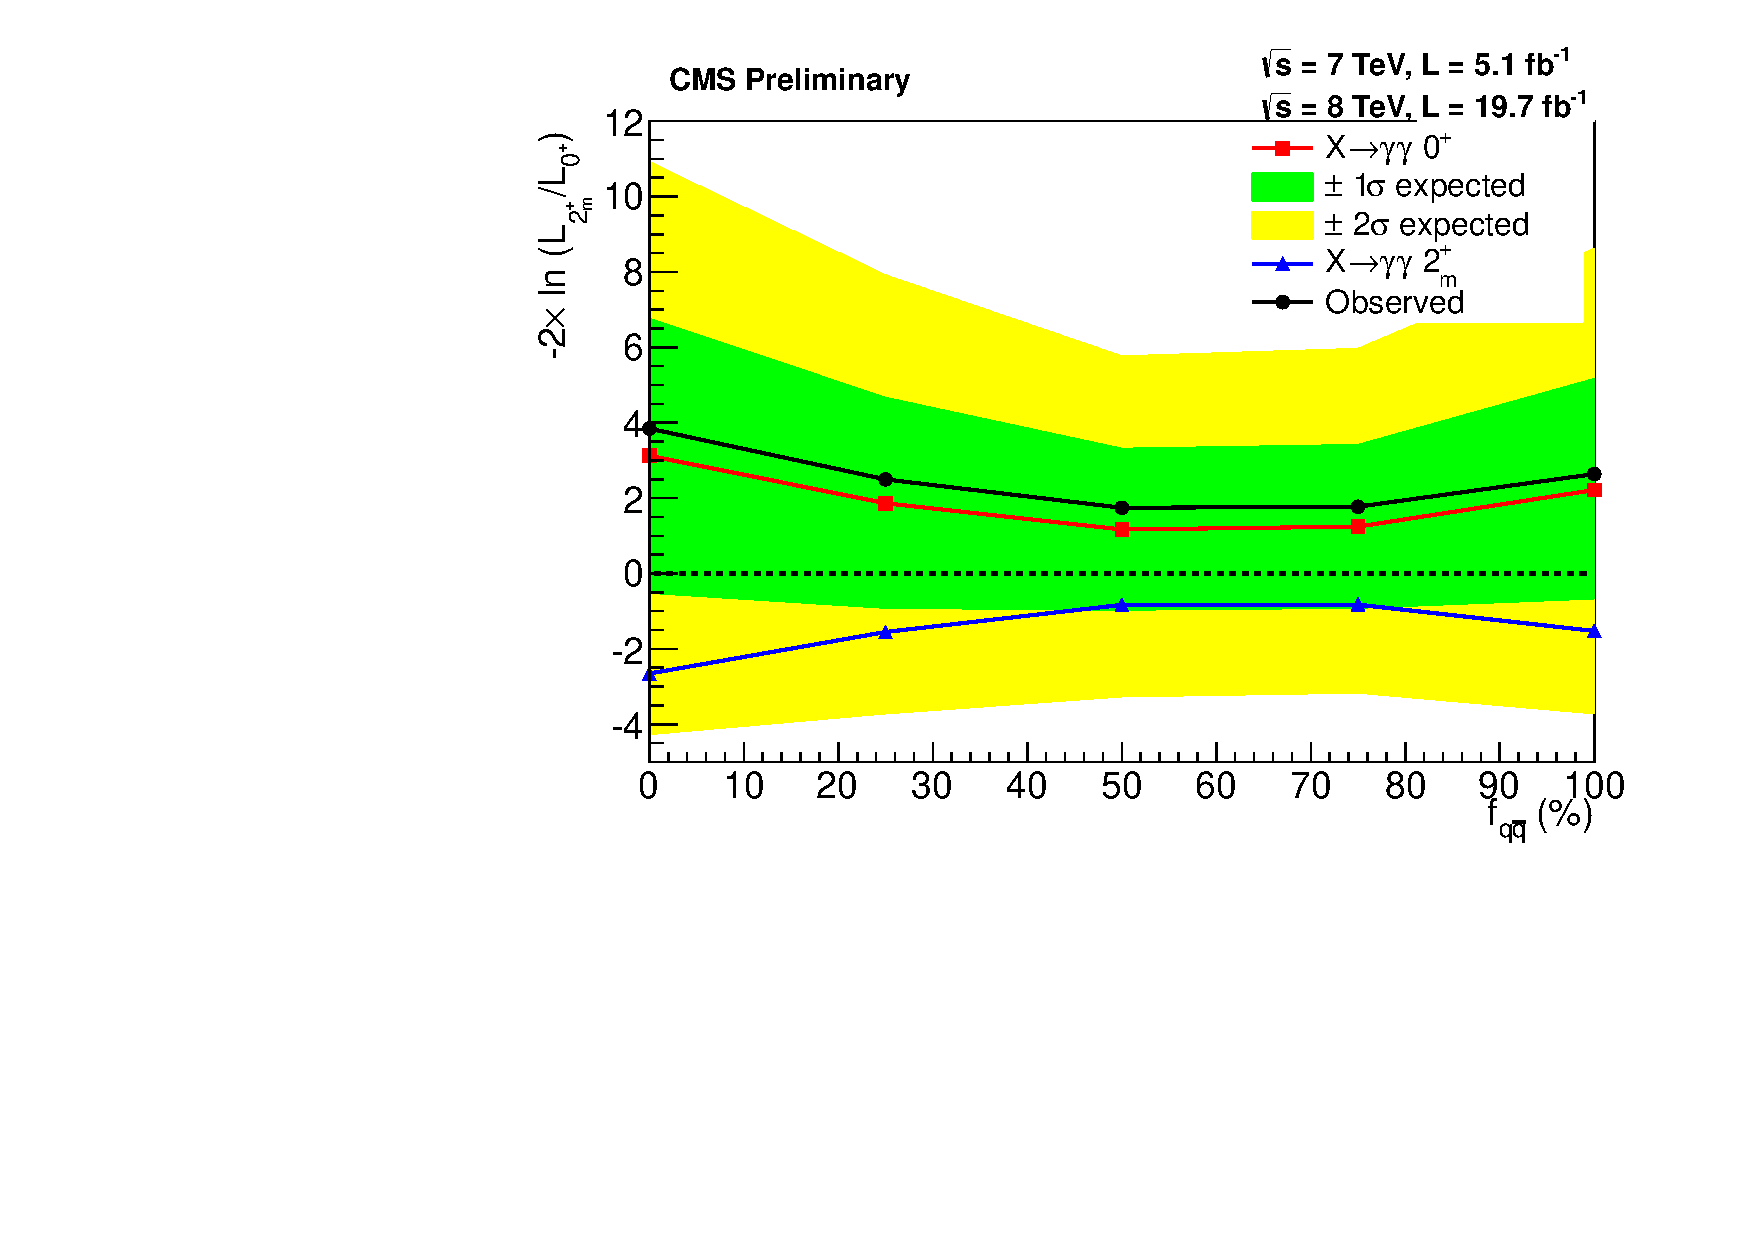
\includegraphics[width=0.8\linewidth]{spin/plots/fqqbar_unblind.pdf}
    \caption{The distribution of the test statistic for pseudo experiments thrown under the SM, \zerop, hypothesis (red) and the \emph{graviton-like}, \twomp, hypothesis (blue) as a function of the fraction of \qqbar production relative to $gg$ production. The observed distribution in the data is shown by the black points.}
    \label{fig:qqbar}
  \end{center}
\end{figure}



